
% ----------------------------------------------------------------------
%  Set the document class
% ----------------------------------------------------------------------
\documentclass[11pt,a4paper,twoside]{article}

% ----------------------------------------------------------------------
% Define external packages, language, margins, fonts and new commands
% ----------------------------------------------------------------------
%\input{preamble}
\usepackage{amsmath}
\usepackage{mathtools}
\usepackage[utf8]{inputenc}   % <<<<< Linux
\usepackage[english]{babel} % <<<<< English
\usepackage{notoccite}
\usepackage[skip=0.5\baselineskip]{caption}
\hyphenation{GTKWave}
\usepackage{listings}
\usepackage[all]{nowidow}

%blind text
\usepackage{lipsum}

\usepackage{graphicx}
\graphicspath{{./}{../../figlib/}{../mat/}{../sim/}}
\def\FontLn{% 16 pt normal
  \usefont{T1}{phv}{m}{n}\fontsize{16pt}{16pt}\selectfont}
\def\FontLb{% 16 pt bold
  \usefont{T1}{phv}{b}{n}\fontsize{16pt}{16pt}\selectfont}
\def\FontMn{% 14 pt normal
  \usefont{T1}{phv}{m}{n}\fontsize{14pt}{14pt}\selectfont}
\def\FontMb{% 14 pt bold
  \usefont{T1}{phv}{b}{n}\fontsize{14pt}{14pt}\selectfont}
\def\FontSn{% 12 pt normal
  \usefont{T1}{phv}{m}{n}\fontsize{12pt}{12pt}\selectfont}

% Use Arial font as default
%
\renewcommand{\rmdefault}{phv}
\renewcommand{\sfdefault}{phv}
\usepackage{geometry}	
\geometry{verbose,tmargin=2.5cm,bmargin=2.5cm,lmargin=2.5cm,rmargin=2.5cm}

%\usepackage{setspace}
%\renewcommand{\baselinestretch}{1.5}

\usepackage[pdftex]{hyperref} % enhance documents that are to be
                              % output as HTML and PDF
\hypersetup{colorlinks,       % color text of links and anchors,
                              % eliminates borders around links
%            linkcolor=red,    % color for normal internal links
            linkcolor=black,  % color for normal internal links
            anchorcolor=black,% color for anchor text
%            citecolor=green,  % color for bibliographical citations
            citecolor=black,  % color for bibliographical citations
%            filecolor=magenta,% color for URLs which open local files
            filecolor=black,  % color for URLs which open local files
%            menucolor=red,    % color for Acrobat menu items
            menucolor=black,  % color for Acrobat menu items
%            pagecolor=red,    % color for links to other pages
            pagecolor=black,  % color for links to other pages
%            urlcolor=cyan,    % color for linked URLs
            urlcolor=black,   % color for linked URLs
	          bookmarks=true,         % create PDF bookmarks
	          bookmarksopen=false,    % don't expand bookmarks
	          bookmarksnumbered=true, % number bookmarks
	          pdftitle={report},
            pdfauthor={Andre C. Marta},
%            pdfsubject={Thesis Title},
%            pdfkeywords={Thesis Keywords},
            pdfstartview=FitV,
            pdfdisplaydoctitle=true}

\usepackage[numbers,sort&compress]{natbib} % <<<<< References in numbered list [1],[2],...
\usepackage{subcaption} 
\usepackage{mdframed}

\usepackage{float}

%%%%%%%%%%%%%%%%%%%%%%%%%%%%%%%%%%%%%%%%%%%%%%%%%%%%%%%%%%%%%%%%%%%%%%%%
%     Begin Document                                                   %
%%%%%%%%%%%%%%%%%%%%%%%%%%%%%%%%%%%%%%%%%%%%%%%%%%%%%%%%%%%%%%%%%%%%%%%%


\begin{document}

% Set plain page style (no headers, footer with centered page number)
\pagestyle{plain}

% Set roman numbering (i,ii,...) before the start of chapters
%\pagenumbering{roman}

% ----------------------------------------------------------------------
%  Cover page
% ----------------------------------------------------------------------
%%%%%%%%%%%%%%%%%%%%%%%%%%%%%%%%%%%%%%%%%%%%%%%%%%%%%%%%%%%%%%%%%%%%%%%%
%                                                                      %
%     File: Thesis_FrontCover.tex                                      %
%     Tex Master: Thesis.tex                                           %
%                                                                      %
%     Author: Andre C. Marta                                           %
%     Last modified :  2 Jul 2015                                      %
%                                                                      %
%%%%%%%%%%%%%%%%%%%%%%%%%%%%%%%%%%%%%%%%%%%%%%%%%%%%%%%%%%%%%%%%%%%%%%%%

\thispagestyle {empty}

% IST Logo - Signature A
% parameters: bb=llx lly urx ury (bounding box), width=h_length, height=v_length, angle=angle, scale=factor, clip=true/false, draft=true/false. 
\includegraphics[bb=9.5cm 11cm 0cm 0cm,scale=0.29]{IST_A_CMYK_POS}

\begin{center}
%
% Figure (Image or plot)
\vspace{1.0cm}
% height = 50 mm
%\includegraphics[height=50mm]{Figures/Airbus_A350.jpg}

% Title, author and degree
\vspace{1cm}
%{\FontLb Circuit Theory and Electronics Fundamentals} \\ % <<<<< EDIT TITLE
{\FontLb \Huge Lab 3: AC/DC Converter} \\ % <<<<< EDIT TITLE
\vspace{1cm}
%{\FontSn Department of Electrical and Computer Engineering, Técnico, University of Lisbon} \\ % <<<<< EDIT COURSE
{\FontSn \Large Circuit Theory and Electronics Fundamentals} \\ % <<<<< EDIT COURSE
{\FontSn \large Master's programme in Engineering Physics, Técnico, University of Lisbon} \\ % <<<<< EDIT COURSE
\vspace{1cm}
%{\FontSn Example Laboratory Report} \\
{\FontSn Diogo Costa | 96187} \\
{\FontSn Ana Sousa | 96508} \\
{\FontSn Isabel Alexandre | 96537} \\
\vspace{1cm}
{\FontSn May 05, 2021} \\ % <<<<< EDIT DATE (corresponds to date of oral examination)
%
\end{center}

% MEFT = Master's programme in Engineering Physics



% ----------------------------------------------------------------------
% Dedication page (optional)
% ----------------------------------------------------------------------
%\input{dedication} 
%\cleardoublepage

% ----------------------------------------------------------------------
%  Acknowledgments (optional)
% ----------------------------------------------------------------------
%\input{acknowledgements}
%\cleardoublepage

% ----------------------------------------------------------------------
%  Abstract (both in English and Portuguese)
% ----------------------------------------------------------------------
%\input{resumo} 
%\cleardoublepage

%\input{abstract} 

% ----------------------------------------------------------------------
%  Table of contents, list of tables, list of figures and nomenclature
% ----------------------------------------------------------------------

% Table of contents
%
\tableofcontents

% List of tables
%\addcontentsline{toc}{section}{\listtablename}
%\listoftables
%\cleardoublepage 

% List of figures
%\addcontentsline{toc}{section}{\listfigurename}
%\listoffigures
%\cleardoublepage 

% Set arabic numbering (1,2,...) after preface
%
%\setcounter{page}{1}
%\pagenumbering{arabic}

% ----------------------------------------------------------------------
%  Body
% ----------------------------------------------------------------------

\newpage

\section{Introduction}
\label{sec:introduction}

The main objective of this laboratory assignment is to design a bandpass filter, using an OP-AMP. This filter should be centered at $1\;kHz$ and produce a gain of $40\;dB$ at this frequency. There are also some limitations in terms of resources: maximum 3 $1\;k\Omega$ resistors, 3 $10\;k\Omega$ resistors, 3 $100\;k\Omega$ resistors, 3 $220\;nF$ capacitors and 3 $1\;\mu F$ capacitors. 

The secondary goal is to achieve the best performance at the lowest cost. This is quantified by maximizing the following function:

\begin{equation}
  M = \frac{1}{cost (gainDeviation + centralFrequencyDeviation + 10^{-6})}
\end{equation}

\begin{gather*}
  cost = cost\;of\;resistors + cost\;of\;capacitors + cost\;of\;transistors + cost\;of\;diodes \\
  cost\;of\;resistors = 1 MU/k\Omega \\
  cost\;of\;capacitors = 1 MU/\mu F \\
  cost\;of\;diodes = 0.1 MU/diode \\
  cost\;of\;transistors = 0.1 MU/transistor
\end{gather*}

In Section~\ref{sec:laboratory} a basic filter circuit is introduced and the study performed in the laboratory, using this circuit, is presented. This is followed by Section~\ref{sec:simulation}, where the same circuit is simulated. Furthermore, in an effort to improve our results, an optimized circuit is obtained and presented. A theoretical analysis is then performed, considering either circuit, in Section~\ref{sec:analysis}. The results obtained for the optimized circuit via simulation and theoretical analysis are compared in Section~\ref{sec:conclusion}. Here, $M$ is presented, allowing for some considerations to be made about the studies performed. The simulation was run on {\bf Ngspice} and the theoretical calculations were performed with {\bf Octave}.

%The main objective of this laboratory assignment is to design an audio amplifier. This circuit should be able to amplify $10\;mV$ of alternating current at a wide range of frequencies. To this purpose, three types of components will be employed: resistors, capacitors and transistors.
%The secondary goal is to achieve the best performance at the lowest cost. This is quantified by maximizing the following function:
%\begin{equation}
%  M = \frac{voltageGain \cdot bandwidth}{cost \cdot lowerCutoffFrequency}
%\end{equation}
%\begin{gather*}
%  cost = cost\;of\;resistors + cost\;of\;capacitors + cost\;of\;transistors \\
%  cost\;of\;resistors = 1 MU/k\Omega \\
%  cost\;of\;capacitors = 1 MU/\mu F \\
%  cost\;of\;transistors = 0.1 MU/transistor
%\end{gather*}
%In Section~\ref{sec:simulation}, the amplifier is presented and its behaviour is studied using a simulation. This is followed by a theoretical analysis of the circuit, in Section~\ref{sec:analysis}. Both are compared in the final section, Section ~\ref{sec:conclusion}. Here, $M$ is also presented, allowing for some considerations to be made about the circuit designed. The simulation was run by using {\bf Ngspice} and the theoretical calculations were performed with {\bf Octave}.


\newpage

\section{Simulation Analysis}
\label{sec:simulation}

\subsection{Simple circuit}

\begin{figure}[H]
\centering
\includegraphics[width=0.6\textwidth]{gain_sim}
\caption{Data collected versus simulated data}
\label{data_graph_sim}
\end{figure}

It is obvious, from the above graph, that there are slight deviations between the real data and the simulated data, as expected. This can be due to any number of experimental causes:

\begin{itemize}

\item Errors in the peak to peak amplitude determined by the oscilloscope

\item Errors in the resistors used in the lab (had gold tolerance)

\item Errors in the capacitors used in the lab

\item For the $500\;\Omega$ resistor, two $1\;k\Omega$ resistors were employed, in parallel

\item All signals went through the breadboard

\item $V_{CC}$ was not exactly $10\;V$ and $V_{EE}$ was not exactly $-10\;V$

\item Discrepancies in the {\bf Ngpisce} models

\end{itemize}

Using these parameters, the following was obtained:

\begin{table}[H]
  \centering
  \begin{tabular}{|c|c|}
    \hline
        {\bf Name} & {\bf Value} \\
        \hline
        \hline
        \input{lab}
        \hline
  \end{tabular}
  \caption{Results}
  \label{sim_results}
\end{table}

\begin{figure}[H]
\centering
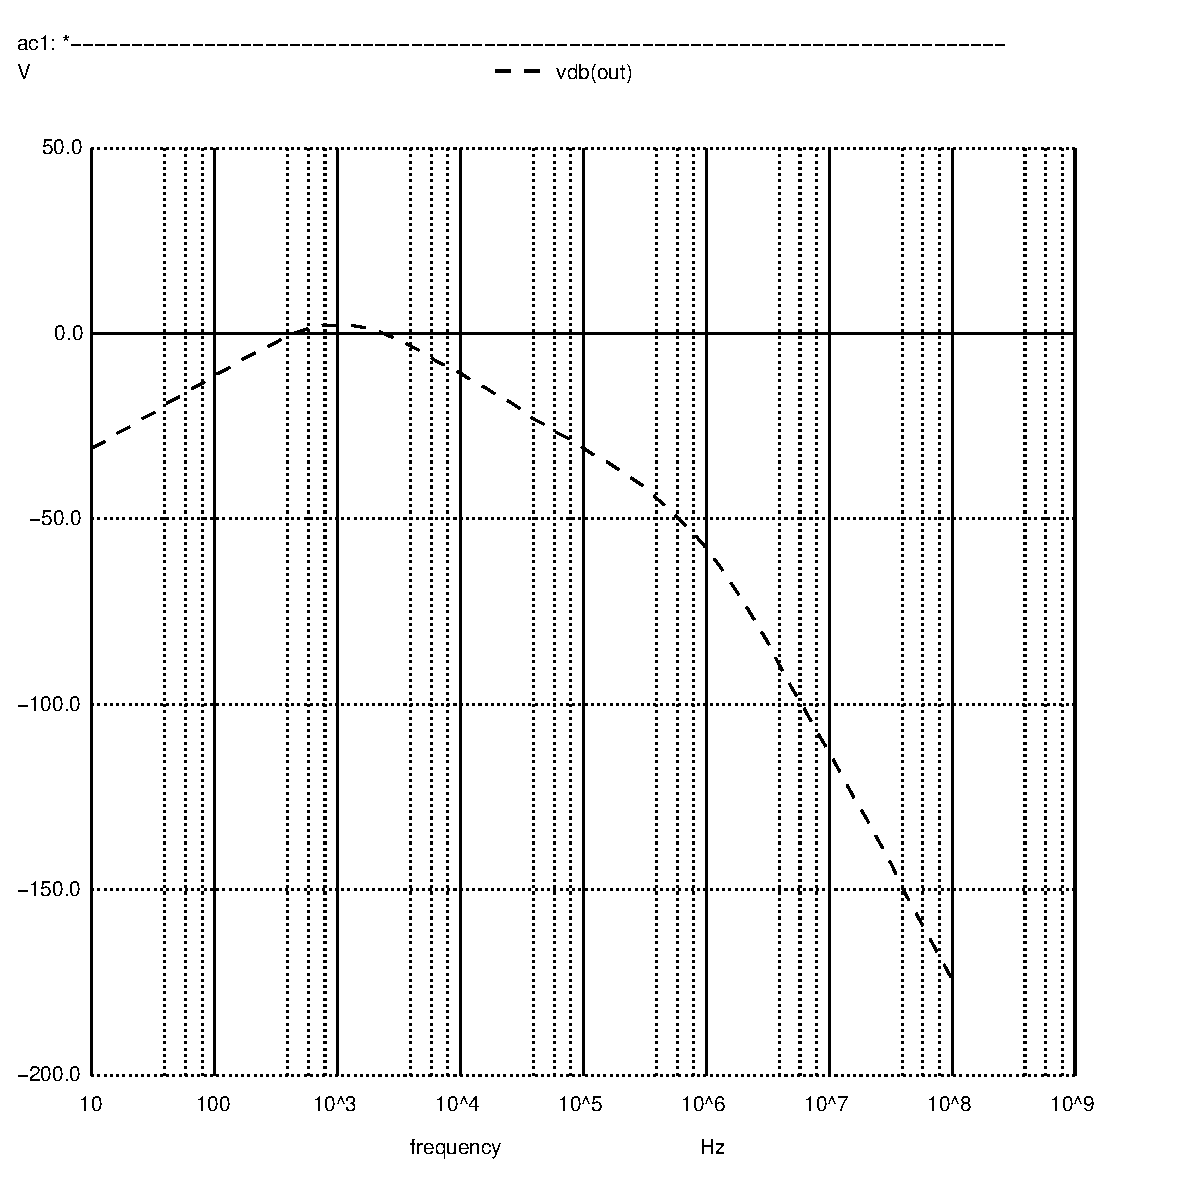
\includegraphics[width=0.6\textwidth]{vo1f}
\caption{Frequency response - gain}
\end{figure}

\begin{figure}[H]
\centering
\includegraphics[width=0.6\textwidth]{vo1f_phase}
\caption{Frequency response - phase}
\end{figure}

\subsection{Optimized circuit}

\begin{table}[H]
  \centering
  \begin{tabular}{|c|c|}
    \hline
        {\bf Name} & {\bf Value} \\
        \hline
        \hline
        $f_c\; (Hz)$ & 262.77028969352676 \\ 
 \hline 
$gain(f_c)\; (dB)$ & 38.19408 \\ 
 \hline 
$z_{in}$ & 0.4999899 + i ( -0.159204 ) \\ 
 \hline 
$z_{out}$ & 0.341692 + i ( -0.233043 ) \\ 
 \hline 

        \hline
  \end{tabular}
  \caption{Results}
  \label{sim_mb_results}
\end{table}

\begin{figure}[H]
\centering
\includegraphics[width=0.6\textwidth]{vo1f_mb}
\caption{Frequency response - gain}
\end{figure}

\begin{figure}[H]
\centering
\includegraphics[width=0.6\textwidth]{vo1f_mb_phase}
\caption{Frequency response - phase}
\end{figure}


\section{Theoretical Analysis}
\label{sec:analysis}

In this section, the circuit depicted in Figure~\ref{circuit} is analysed with two different methods, so as to determine how it behaves, theoretically, both in terms of current in each branch and potential difference between nodes.

To provide for common ground between the theoretical analysis and the simulation run, and to allow for easy comparison, we presented all relevant parameters of the system in three similar tables, in Subsections \ref{sec:mesh}, \ref{sec:node} and \ref{sec:op_point}. The first two were produced using {\bf Octave} and the latter was generated by {\bf Ngspice}.

\subsection{Mesh analysis method}
\label{sec:mesh}

The first method considered is the Mesh analysis method, considering the four meshes present in the circuit. Each mesh is given a label ($\alpha$, $\beta$, $\gamma$ and $\delta$) and an arbitrary direction for the current to flow in, as the below figure shows.

\begin{figure}[H]
  \centering
  \includegraphics[width=0.5\linewidth]{mesh1.pdf}
  \caption{Mesh analysis}
  \label{mesh_fig}
\end{figure}

\newpage

By inspection:

\begin{equation}
  \begin{cases}
    I_{\alpha} = I_d \\
    I_{\beta} = I_b
  \end{cases}
\end{equation}

Applying KVL to the two remaining meshes:

\begin{equation}
  \begin{cases}
    V_a + R_4 (I_\gamma + I_\delta) + R_3 (I_\gamma - I_\beta) + R_1 I_\gamma = 0 \\
    V_c + R_7 I_\delta + R_6 I_\delta + R_4 (I_\delta + I_\gamma) = 0
  \end{cases}
\end{equation}

The conditional sources behave as:

\begin{equation}
  \begin{cases}
  I_b = k_b V_b \\
  V_c = k_c I_c = - k_c I_\delta
  \end{cases}
\end{equation}

Lastly, by Ohm's Law

\begin{equation}
  V_b = R_3 (I_\beta - I_\gamma)
\end{equation}

Manipulating these equations and solving them using {\bf Octave} yields:

%\begin{equation}
%  \begin{bmatrix}
%  1 & 0 & 0 & 0 \\
%  0 & 1-k_b R_3 & k_b R_3 & 0 \\
%  0 & -R_3 & R_1+R_3+R_4 & R_4 \\
%  0 & 0 & R_4 & R_4+R_6+R_7-k_c
%  \end{bmatrix}
%  \begin{bmatrix}
%  I_\alpha \\
%  I_\beta \\
%  I_\gamma \\
%  I_\delta
%  \end{bmatrix}
%  =
%  \begin{bmatrix}
%  I_d \\
%  0 \\
%  -V_a \\
%  0
%  \end{bmatrix}
%\end{equation}

%Solving this system using Octave,

\begin{table}[H]
  \centering
  \begin{tabular}{|c|c|}
    \hline
        {\bf Name} & {\bf Value} \footnotemark \\
        \hline
        \hline
        $I_\alpha\;(A)$ & $0.001000$ \\ 
\hline
$I_\beta\;(A)$ & $-0.000251$ \\ 
\hline
$I_\gamma\;(A)$ & $-0.000240$ \\ 
\hline
$I_\delta\;(A)$ & $-0.000969$ \\ 
\hline
$I_c\;(A)$ & $0.000969$ \\ 
\hline
$I_b\;(A)$ & $-0.000251$ \\ 
\hline
$V_2\;(V)$ & $5.070727$ \\ 
\hline
$V_3\;(V)$ & $4.825468$ \\ 
\hline
$V_4\;(V)$ & $4.304579$ \\ 
\hline
$V_5\;(V)$ & $4.860091$ \\ 
\hline
$V_6\;(V)$ & $8.720760$ \\ 
\hline
$V_7\;(V)$ & $-2.939898$ \\ 
\hline
$V_8\;(V)$ & $-1.950198$ \\ 
\hline
$V_b\;(V)$ & $-0.034623$ \\ 
\hline
$V_c\;(V)$ & $7.799989$ \\ 

        \hline
  \end{tabular}
  \caption{Theoretical results}
  \label{mesh_res}
\end{table}

\footnotetext{The current directions considered here are the ones depicted in Figure~\ref{node_fig}.}

\newpage

\subsection{Node analysis method}
\label{sec:node}

The second method used was the Node analysis method. With this method, it was possible to determine the voltages in the 8 nodes of the circuit. In Figure~\ref{node_fig}, the directions of the currents chosen to do this analysis are represented, as well as the numerical labels that were given to the nodes.

\begin{figure}[H]
  \centering
  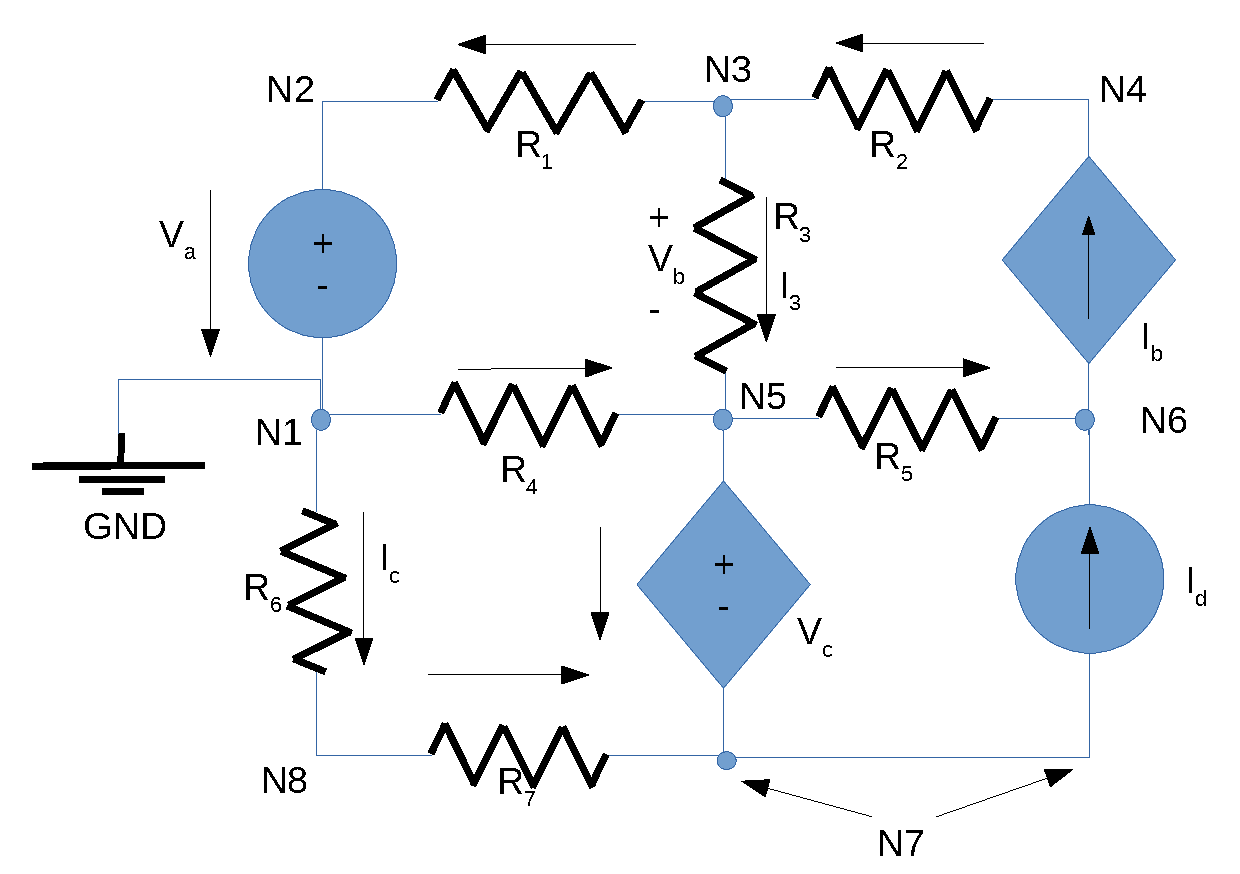
\includegraphics[width=0.5\linewidth]{node.pdf}
  \caption{Node analysis}
  \label{node_fig}
\end{figure}

The node N1 was considered the ground, so:

\begin{equation}
  \begin{cases}
    V_1 = 0 \; V \\
    V_2 = V_a
  \end{cases}
\end{equation}

By applying KCL, it is possible to obtain the following equations:

\begin{equation}
  \begin{cases}
    \frac{V_8}{R_6} + \frac{V_5}{R_4} + \frac{V_3-V_a}{R_1} = 0 \\
    -\frac{V_8}{R_6} - \frac{V_8-V_7}{R_7} = 0 \\
    -\frac{V_3-V_a}{R_1} - \frac{V_3-V_5}{R_3} + \frac{V_4-V_3}{R_2} = 0 \\
    -\frac{V_4-V_3}{R_2} + K_b(V_3-V_5) = 0 \\
    -K_b(V_3-V_5) + \frac{V_5-V_6}{R_5} + I_d = 0
  \end{cases}
\end{equation}

By analysing the dependent voltage source, it is also possible to conclude that

\begin{equation}
  V_5 - V_7 + K_c\frac{V_8}{R_6} = 0
\end{equation}

\newpage

Once again, using {\bf Octave} and the former equations, is possible to determine the voltages in the nodes and the unknown currents and voltages of the circuit:

\begin{table}[H]
  \centering
  \begin{tabular}{|c|c|}
    \hline
        {\bf Name} & {\bf Value} \\
        \hline
        \hline
        $V_2\;(V)$ & $5.070727$ \\ 
\hline
$V_3\;(V)$ & $4.825468$ \\ 
\hline
$V_4\;(V)$ & $4.304579$ \\ 
\hline
$V_5\;(V)$ & $4.860091$ \\ 
\hline
$V_6\;(V)$ & $8.720760$ \\ 
\hline
$V_7\;(V)$ & $-2.939898$ \\ 
\hline
$V_8\;(V)$ & $-1.950198$ \\ 
\hline
$V_b\;(V)$ & $-0.034623$ \\ 
\hline
$I_b\;(V)$ & $-0.000251$ \\ 
\hline
$I_c\;(V)$ & $0.000969$ \\ 
\hline
$V_c\;(V)$ & $7.799989$ \\ 

        \hline
  \end{tabular}
  \caption{Theoretical results}
  \label{node_res}
\end{table} 

The Mesh analysis and the Node analysis are equivalent so, as expected, they produced the same results.




\section{Conclusion}
\label{sec:conclusion}

This laboratory assignment had as the main objective the analysis of the circuit in Figure~\ref{circuit}. That goal was achieved by performing a theoretical analysis, using {\bf Octave}, and a simulation, using {\bf Ngspice}.

In order to easily evaluate the study done, we considered all the parameters presented in previous tables and compared the values obtained by theoretical study and simulation. A very slight deviation is present in some values, but it is not apparent whether it has arised from miscalculations, and is therefore an error, or if it stems from the values being rounded when presented. Nevertheless, we determined, numerically, how significant the deviations are, as shown in Table~\ref{error_res}.

%As one can see there's a very slight deviation in some of the values compared with previous calculations. We proceeded to determine, numerically, how significant these deviations are, as shown in Table~\ref{error_res}. Most of the values are exact ($0\%$) error, and those that aren't have very small errors.

%The theoretical results ($V_t$) do not match perfectly the simulation results ($V_s$). However, the error is quite small, always less than $1\%$.

The circuit is ``simple'' and contains only linear components, so large deviations were not anticipated. These can be due to any number of causes, including but not limited to:

\begin{itemize}
\item floating point arithmetics;
\item different numerical precisions in the different tools employed;
\item propagated errors made when solving the linear system of equations.
\end{itemize}

%The circuit is quite simple and it contains only linear components, so it was not expected that these errors would occur. They have probably arrived due to different number precision in calculations in the two tools used.

%However this error is assumed to be caused by numerical propagated errors made when solving the linear system of equations or simply due to floating point arithmetics. %There's also a certain random error...

All in all, the results obtained were very satisfactory.

\begin{table}[H]
  \centering
  \begin{tabular}{|c|c|c|c|c|}
    \hline
        $V$ & $V_t$ & $V_s$ & $|V_t-V_s|$ & $Error (\%)$ \\
        \hline
        \hline
        $V_2\;(V)$ & $5.070727$ & $5.070727$ & $0.0$ & $0$ \\ 
\hline 
$V_3\;(V)$ & $4.825468$ & $4.827131$ & $0.001663$ & $0.04$ \\ 
\hline 
$V_4\;(V)$ & $4.304579$ & $4.332704$ & $0.028125$ & $0.7$ \\ 
\hline 
$V_5\;(V)$ & $4.860091$ & $4.827131$ & $0.03296$ & $0.7$ \\ 
\hline 
$V_6\;(V)$ & $8.72076$ & $8.648396$ & $0.072364$ & $0.9$ \\ 
\hline 
$V_7\;(V)$ & $-2.939898$ & $-2.91996$ & $0.019938$ & $0.7$ \\ 
\hline 
$V_8\;(V)$ & $-1.950198$ & $-1.93697$ & $0.013228$ & $0.7$ \\ 

        \hline
  \end{tabular}
  \caption{Theoretical results and Simulation results (table produced with {\bf Python}) - The absolute deviation and error presented here are rounded up to one significant digit, for ease of interpretation.}
  \label{error_res}
\end{table}

%\cleardoublepage

% ----------------------------------------------------------------------
%  Bibliography
% ----------------------------------------------------------------------
%\addcontentsline{toc}{section}{\bibname}
%\bibliographystyle{abbrvunsrtnat} % <<<<< SELECT IF USING REFERENCES BY NUMBER (CITATION ORDER)
%\bibliography{../../../BIBfile.bib}

% ----------------------------------------------------------------------
\end{document}
% ----------------------------------------------------------------------
